%!TEX root=../../main.tex

\subsection{Breadth-first search}
As with our results for SSSP, for BFS we will begin with our single-node results before looking at the distributed scenario. Lastly we will compare the two cases.
\subsubsection{Single-Node}
\begin{figure*}
	\begin{subfigure}{0.32\textwidth}
		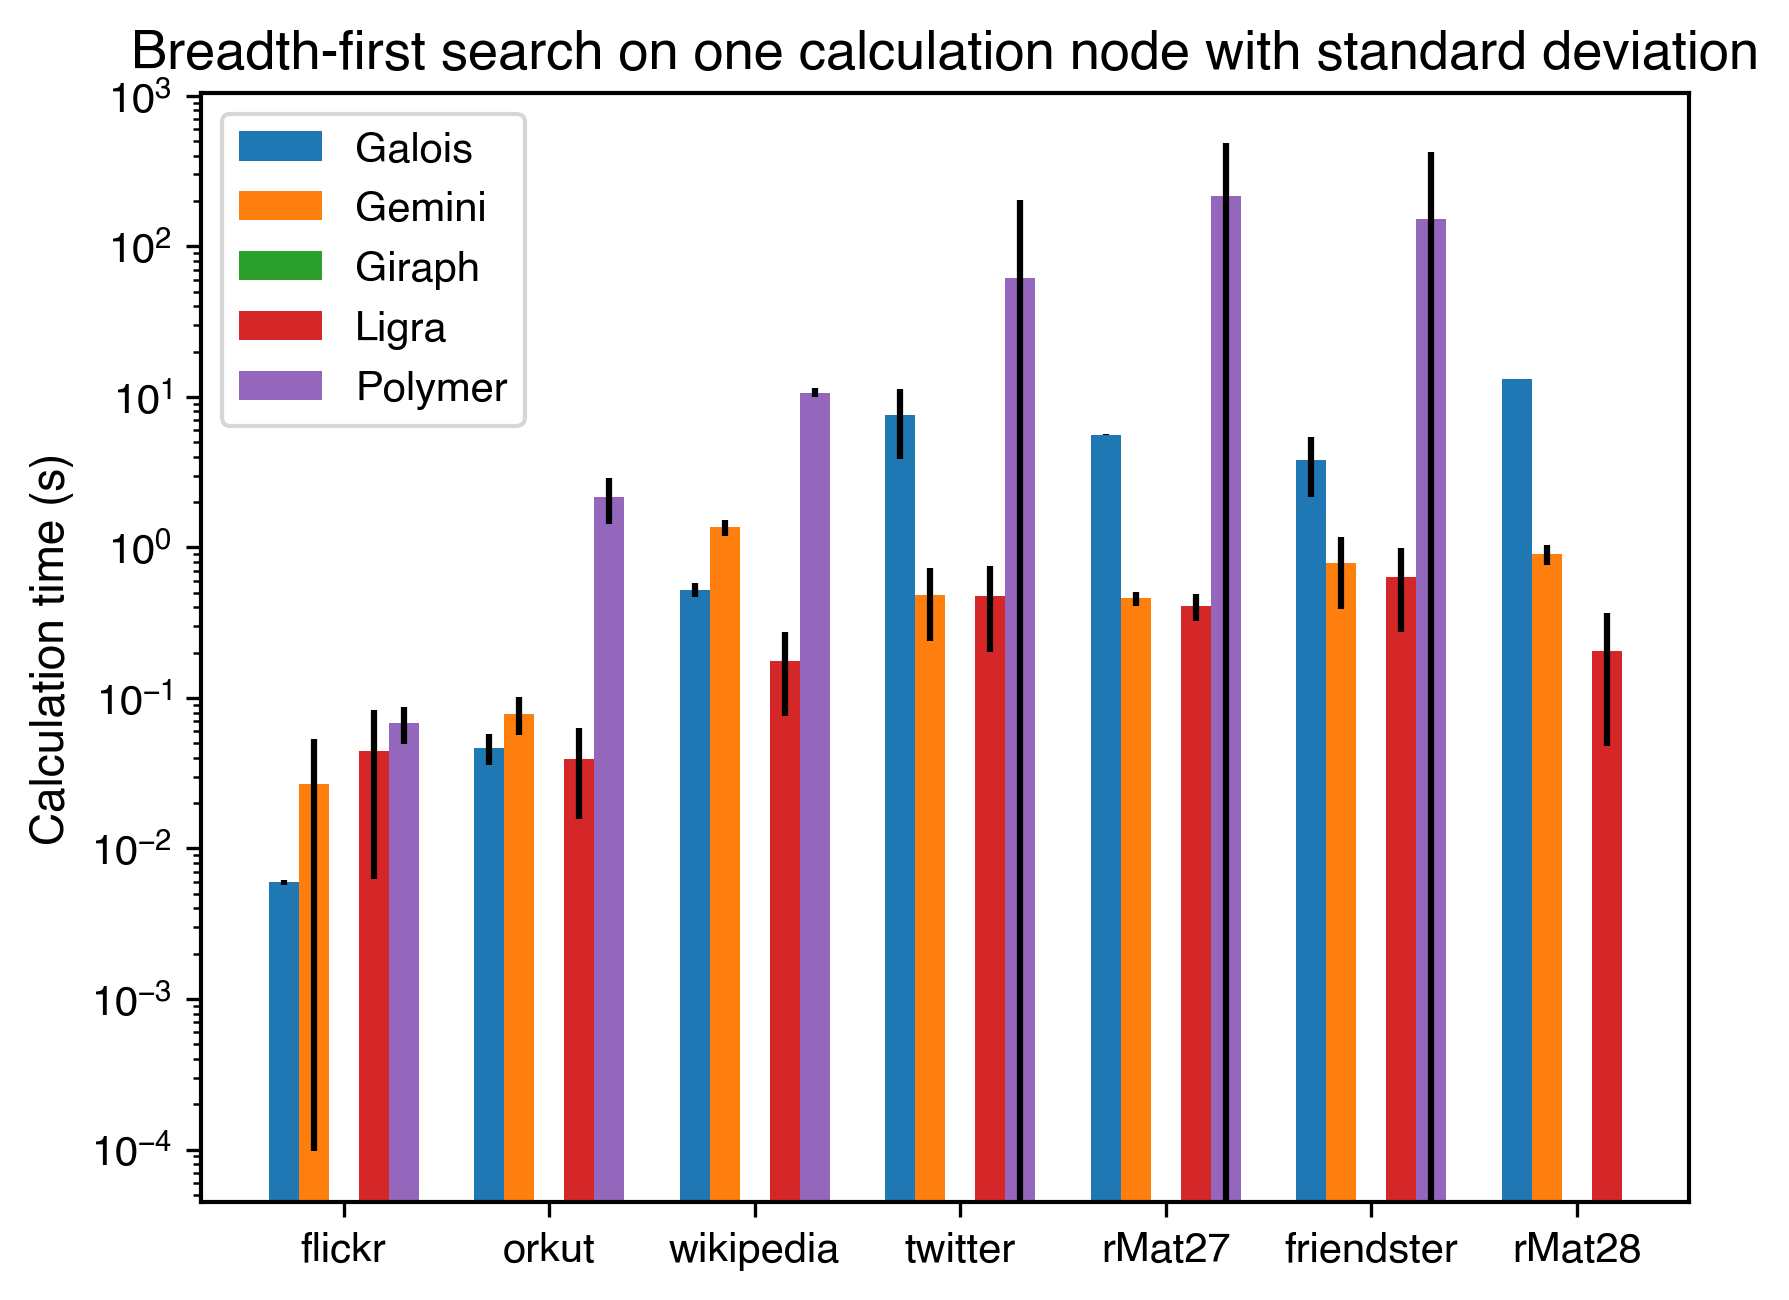
\includegraphics[width=\linewidth]{../../plots/singleNodeBFS_calcTime.png}
		\caption{Calculation time}
		\label{fig:singleNodeBFS_calc}
	\end{subfigure}
	\hfil
	\begin{subfigure}{0.32\textwidth}
		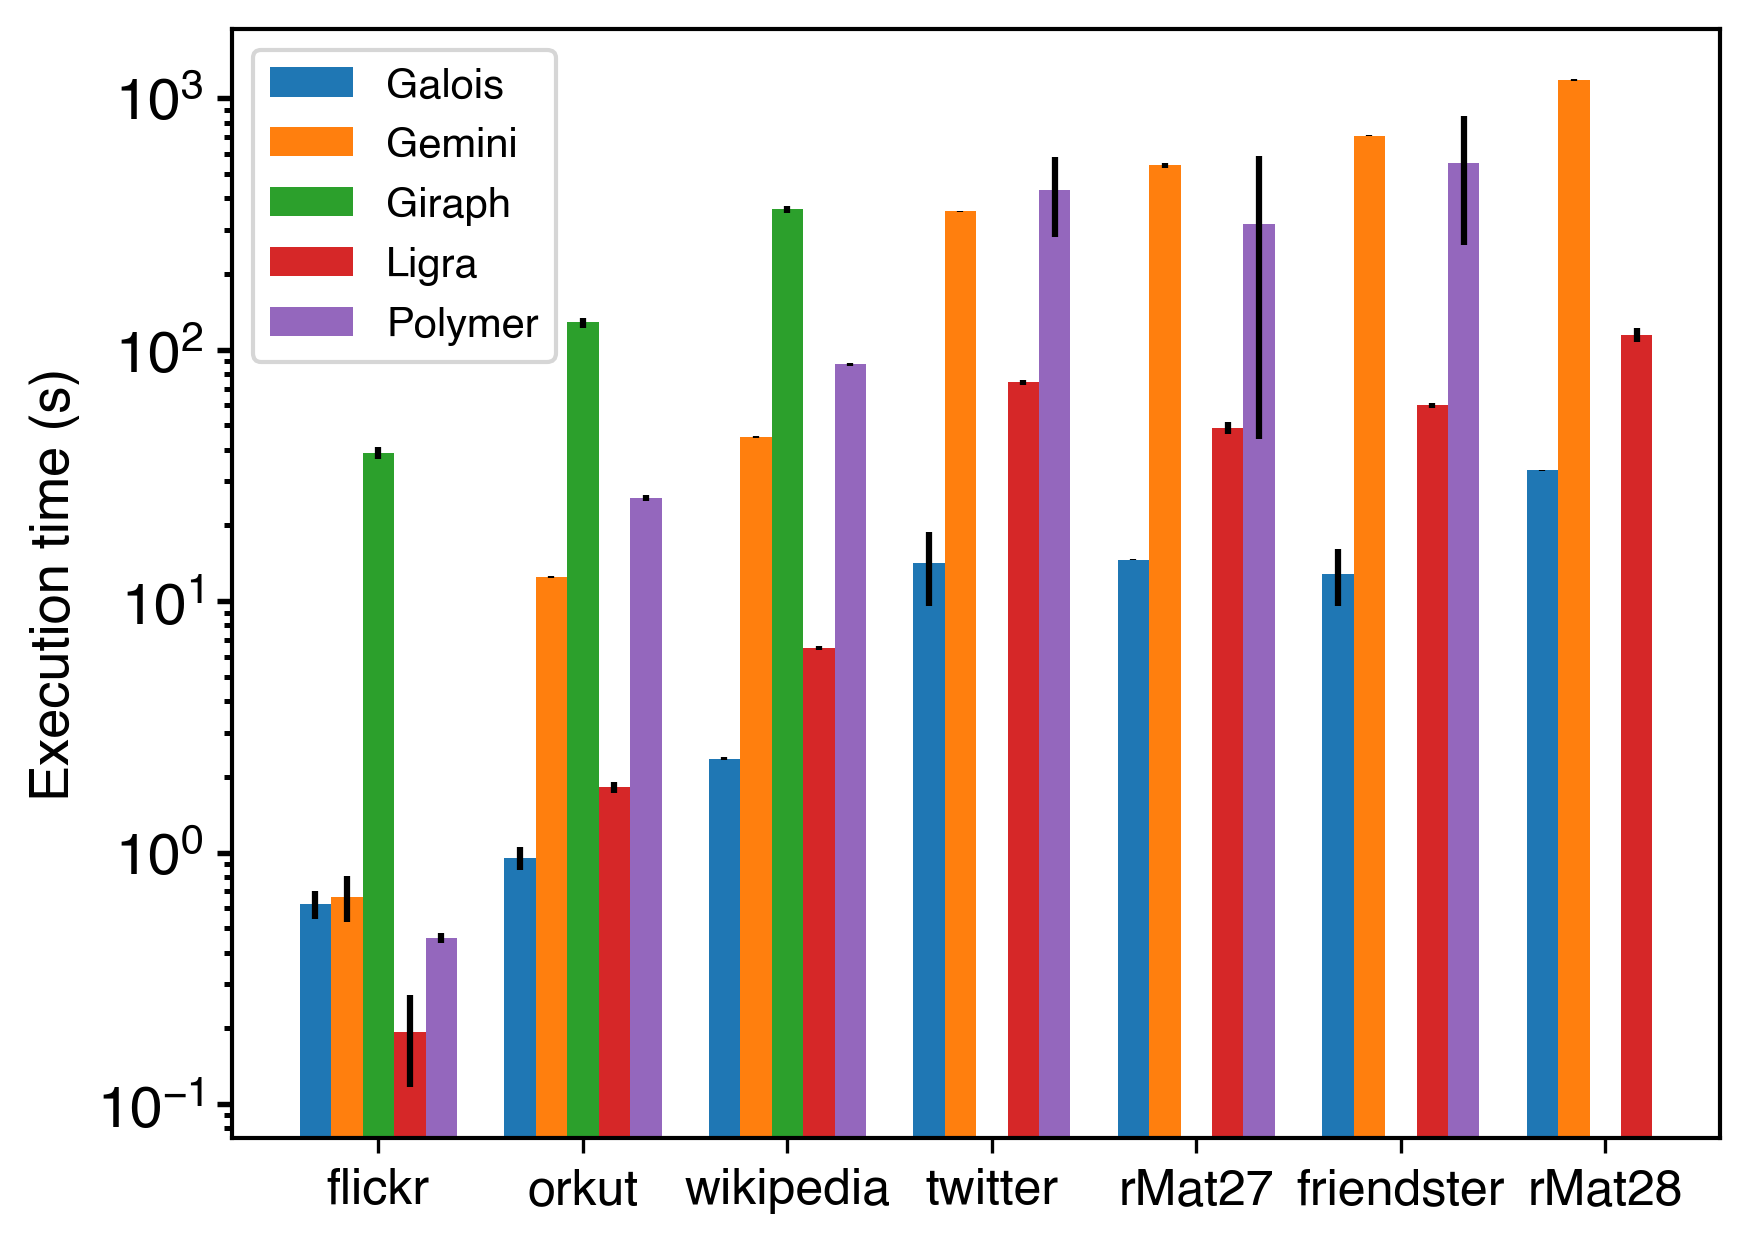
\includegraphics[width=\linewidth]{../../plots/singleNodeBFS_execTime.png}
		\caption{Execution time}
		\label{fig:singleNodeBFS_exec}
	\end{subfigure}
	\hfil
	\begin{subfigure}{0.32\textwidth}
		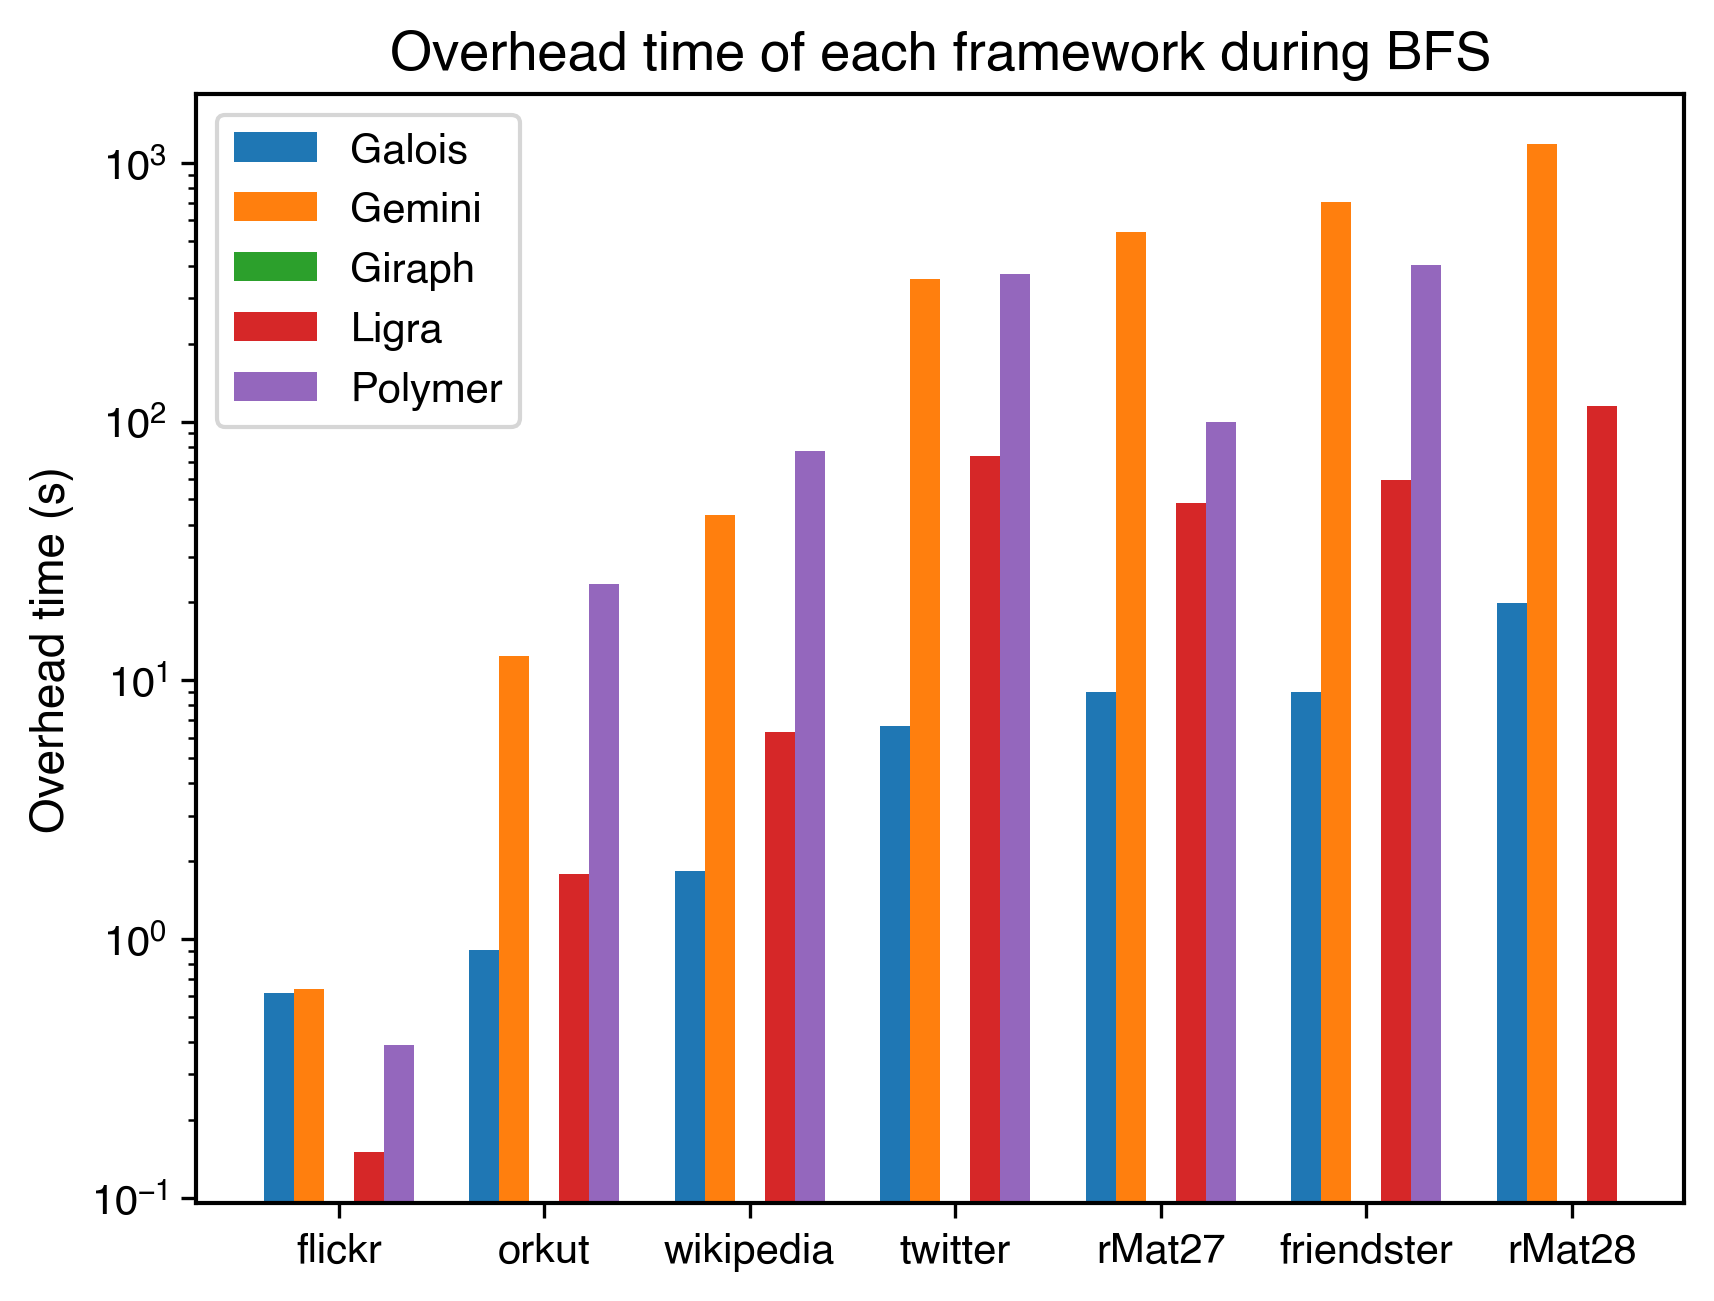
\includegraphics[width=\linewidth]{../../plots/singleNodeBFS_overheadTime.png}
		\caption{Overhead time}
		\label{fig:singleNodeBFS_overheadNormalized}
	\end{subfigure}
	\caption{Average times for BFS on a single computation node, black bars represent one standard deviation in our testing}
\end{figure*}
Just like with SSSP, Giraph ran out of memory ($>$250 GB) on any graph larger than wikipedia. Also, Polymer failed to complete on rMat28. Ligra, that failed during SSSP however completed our benchmark for BFS.

The calculation times provided in \autoref{fig:singleNodeBFS_calc} show Gemini and Ligra to be comparable in their performance. 
Their computation times deviate less than 151ms on all graphs except wikipedia and rMat28, wight Ligra being the faster framework on most graphs.
Ligra is 39ms faster on orkut, 2ms on twitter, 50ms on rMat27 and 151ms on friendster.
In turn, Gemini is 17 ms faster than Ligra on flickr.
Only on wikipedia and rMat28, there is a noticeable difference between the two frameworks. Ligra is 1.2s (7.8$\times$) faster than Gemini on wikipedia and 696ms (4.4$\times$) faster on rMat28.

For the remaining frameworks, we compare to Ligra since it is generally slightly faster than Gemini.
Giraph and Polymer are one to two orders of magnitude slower than both Ligra or Gemini. The only exception to this is Polymer on flickr, here Polymer is just 24ms (35\%) slower than Ligra.
Giraph takes 13$\times$, 32$\times$ and 27$\times$ longer than Ligra on flickr, orkut and wikipedia respectively.
As we said, Polymer is comparable to Ligra on flickr, for the other graphs however, its computation times are even longer than those of Giraph. The upside is though, that Polymer managed -- contrary to Giraph -- to finish computation on some larger graphs.
Polymer takes 55$\times$ longer on orkut, 60$\times$ on wikipedia, 129$\times$ on twitter, 530$\times$ on rMat27 and 240$\times$ on friendster. 
Especially interesting is here the difference between the times of rMat27 and friendster. There are 20\% (439M) edges more in friendster, yet the computation for the synthetic rMat27 takes 42\% longer.

Galois calculation performance is comparable to Gemini or Ligra on the smaller three graphs (flickr, orkut and wikipedia).
On the larger graphs however, Galois is slower than Gemini or Ligra but always faster than Polymer by one order of magnitude.





\subsubsection{Distributed}
\begin{figure*}
	\hfil
	\begin{subfigure}{0.32\textwidth}
		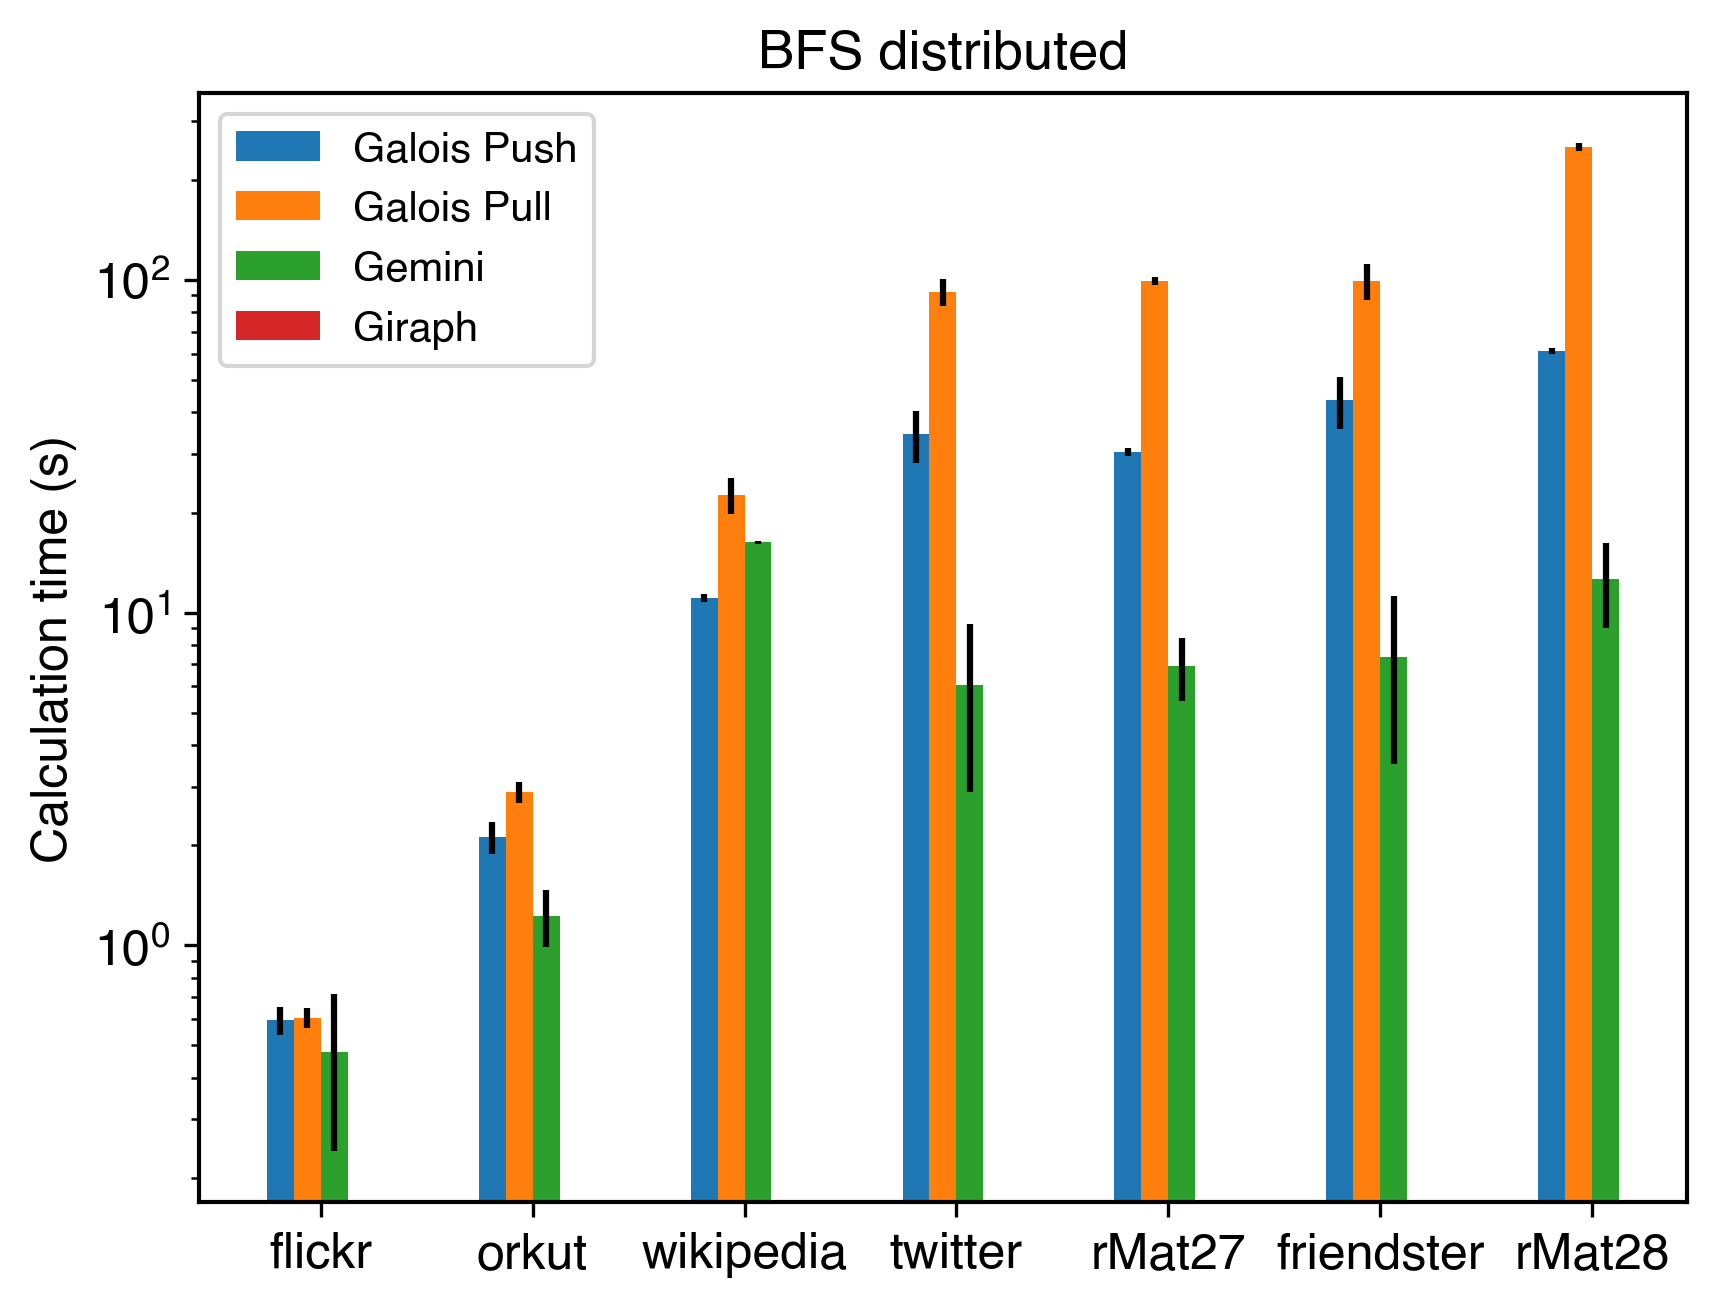
\includegraphics[width=\linewidth]{../../plots/distributedBFS_calcTime.png}
		\caption{Calculation time}
		\label{fig:distributedBFS_calc}
	\end{subfigure}
	\hfil
	\begin{subfigure}{0.32\textwidth}
		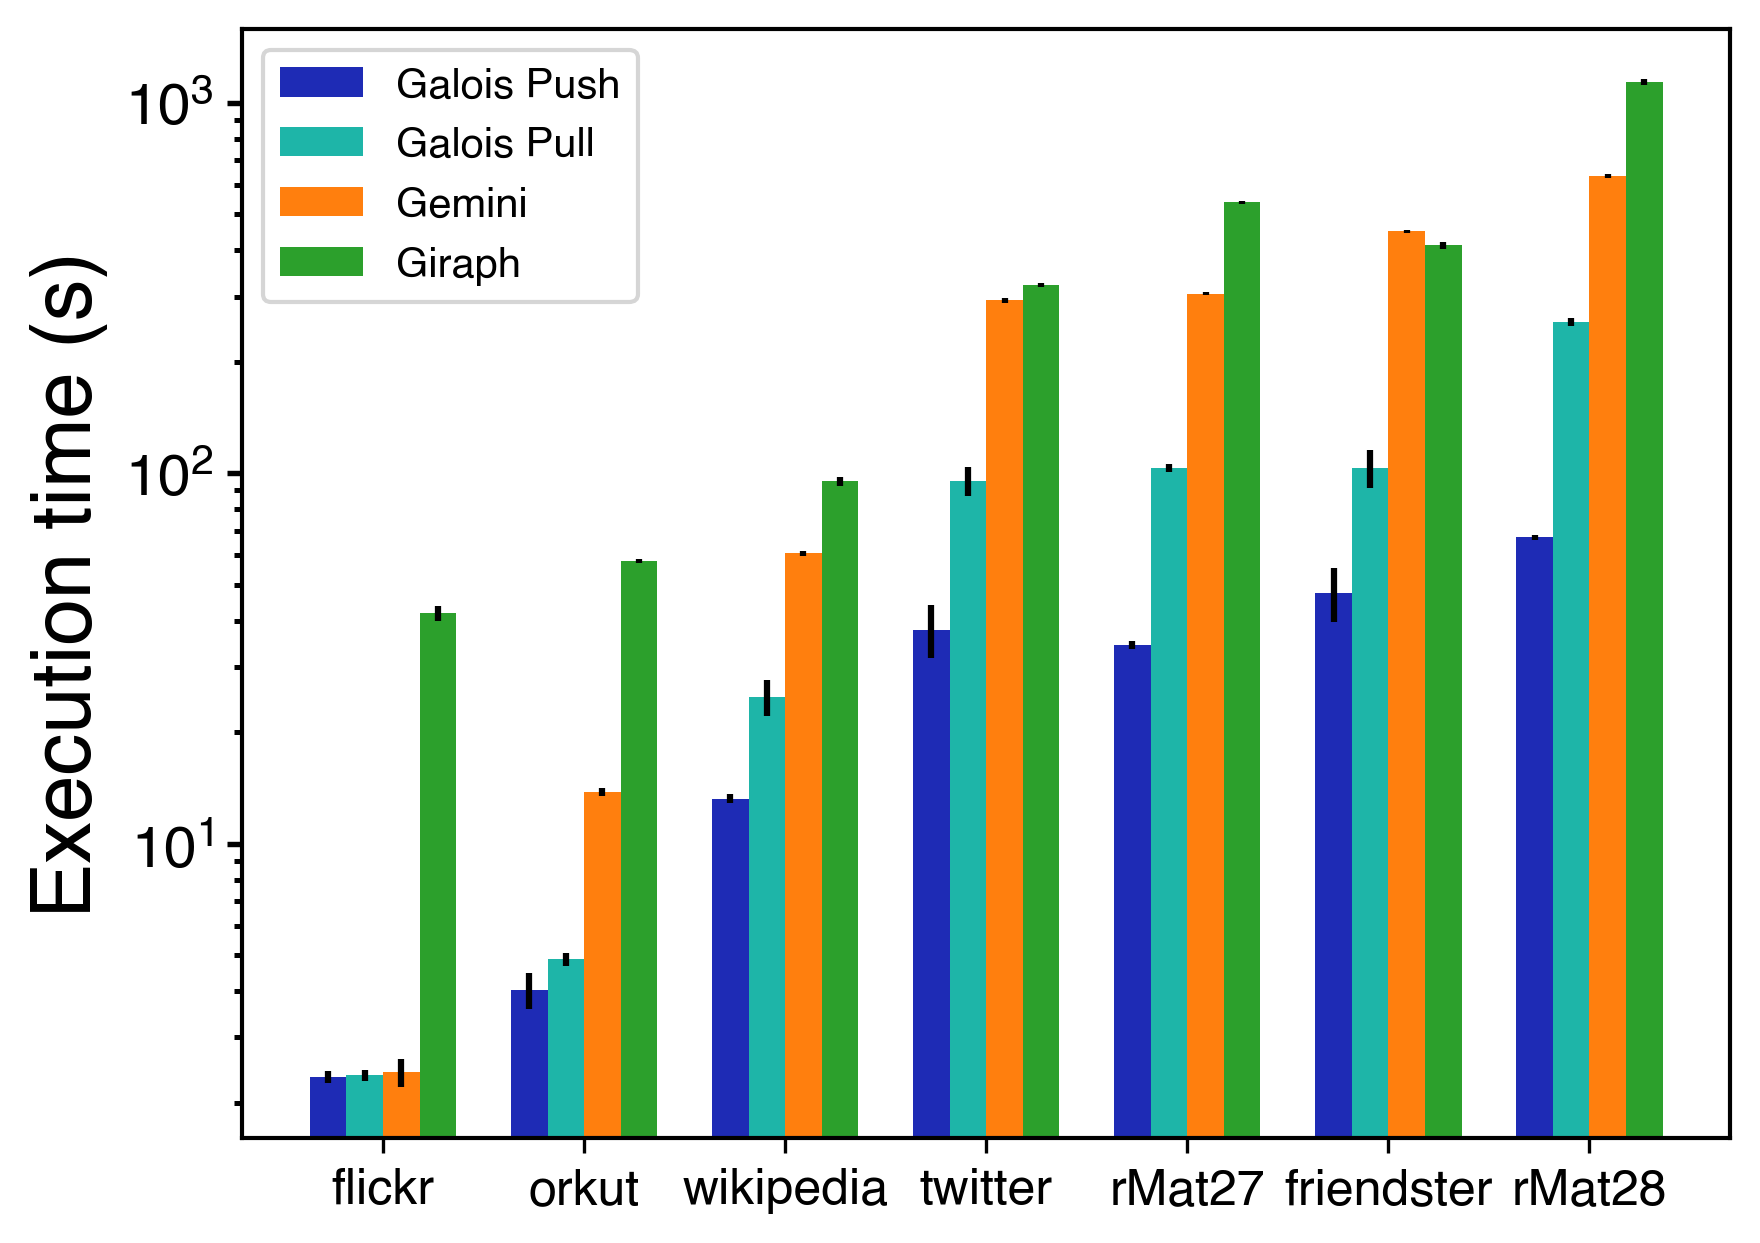
\includegraphics[width=\linewidth]{../../plots/distributedBFS_execTime.png}
		\caption{Execution time}
		\label{fig:distributedBFS_exec}
	\end{subfigure}
	\hfil
	% \begin{subfigure}{0.3\textwidth}
	% 	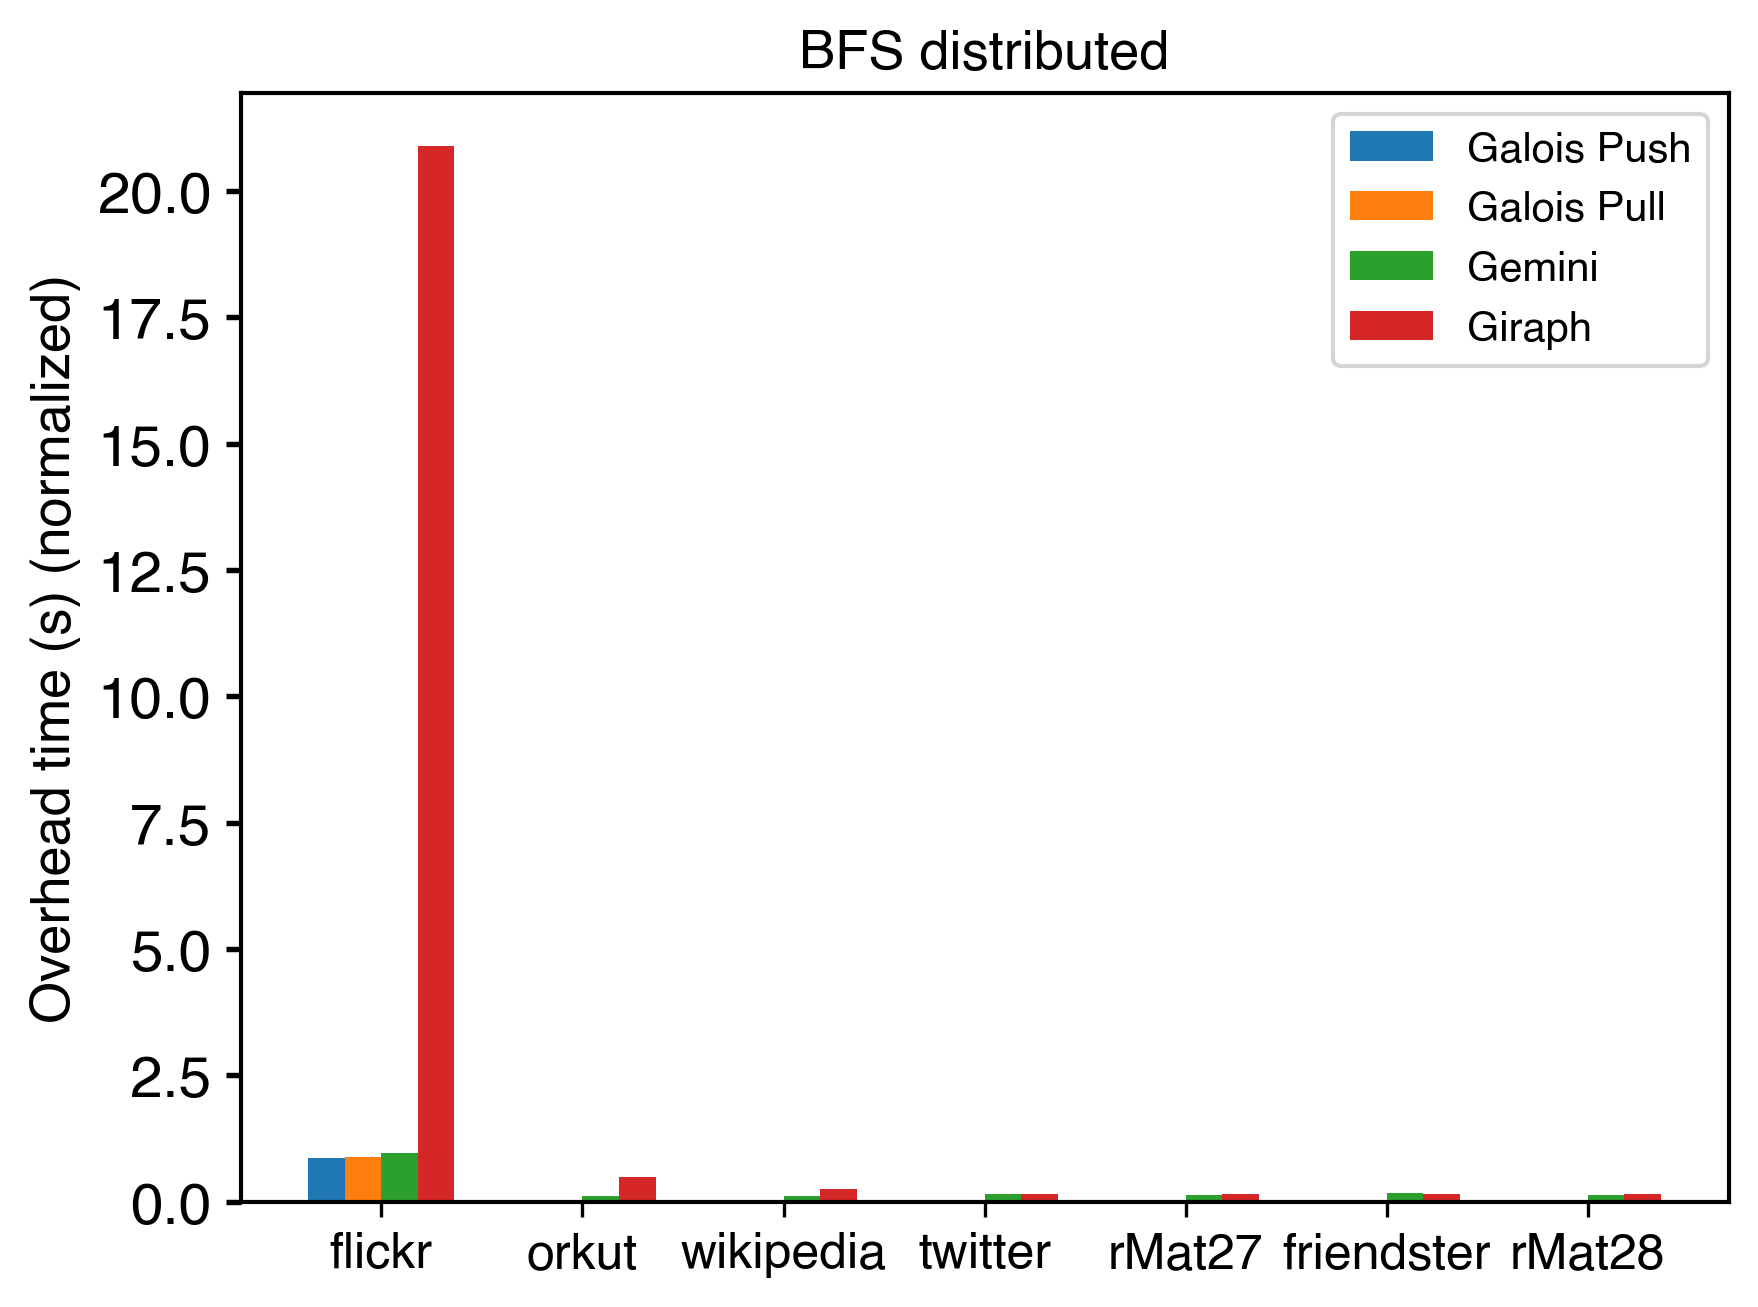
\includegraphics[width=\linewidth]{../../plots/distributedBFS_overheadTimeNormalized.png}
	% 	\caption{Overhead time normalized by the graph size in million edges}
	% 	\label{fig:distributedBFS_overheadNormalized}
	% \end{subfigure}
	\caption{Average times for BFS on the distributed cluster, black bars represent one standard deviation in our testing}
	\label{fig:distributedBFS}
\end{figure*}
For both the calculation and the execution times, Breadth-First Search shows similar behaviour as the distributed SSSP test case. This is expected since both are graph traversal algorithms starting in one source vertex.
Hence, calculation complexity for each vertex and communication overhead is similar.
All measurements can be seen in \autoref{fig:distributedBFS}.

First, the calculation times in \autoref{fig:distributedBFS_calc}. It shows Giraph having the shortest calculation times on the real-world graphs, while Giraph's calculatin times on both rMat27 and rMat28 are the worst of all frameworks.

Comparing the execution times in \autoref{fig:distributedBFS_exec} results in the same findings as with SSSP.
While Gemini can compete with Galois on the small flickr graph, moving to larger data sets shows the worse performance of Gemini compared to Galois.

Much like when running SSSP, Giraph is slowest on all but one graph. Only on friendster is Gemini marginally slower, which was also the case for SSSP.

Both Galois implementations are again similar to the behaviour on SSSP.
Galois Push is generally faster than the Pull alternative while both Push and Pull versions are faster than Gemini and Giraph across all graphs.
This makes Galois Push the clear winner for distributed BFS.

